\subsection{Derived quantities} \label{subsec:DerivedQuantities}
The value of inductance, capacitance or resistance can be calculated once the impedance of the DUT is known, along with the dissipation and quality factor. This chapter will show how this can be achieved. Consider that in section \ref{sec:ImpedanceAnalysis} where the impedance of a DUT could be written in the rectangular form $Z = R \pm jX$. The $jX$ term represents the capacitive, or inductive, reactance that could be used to find the inductance or capacitance value of the DUT.

To find $jX$ consider the circuit on figure \refq{fig:4_1_1_CapCircuit} with a voltage source, $v(t)$, connected across a capacitor and a current $i(t)$ flowing in the circuit. 
\begin{figure}[H]
    \centering
    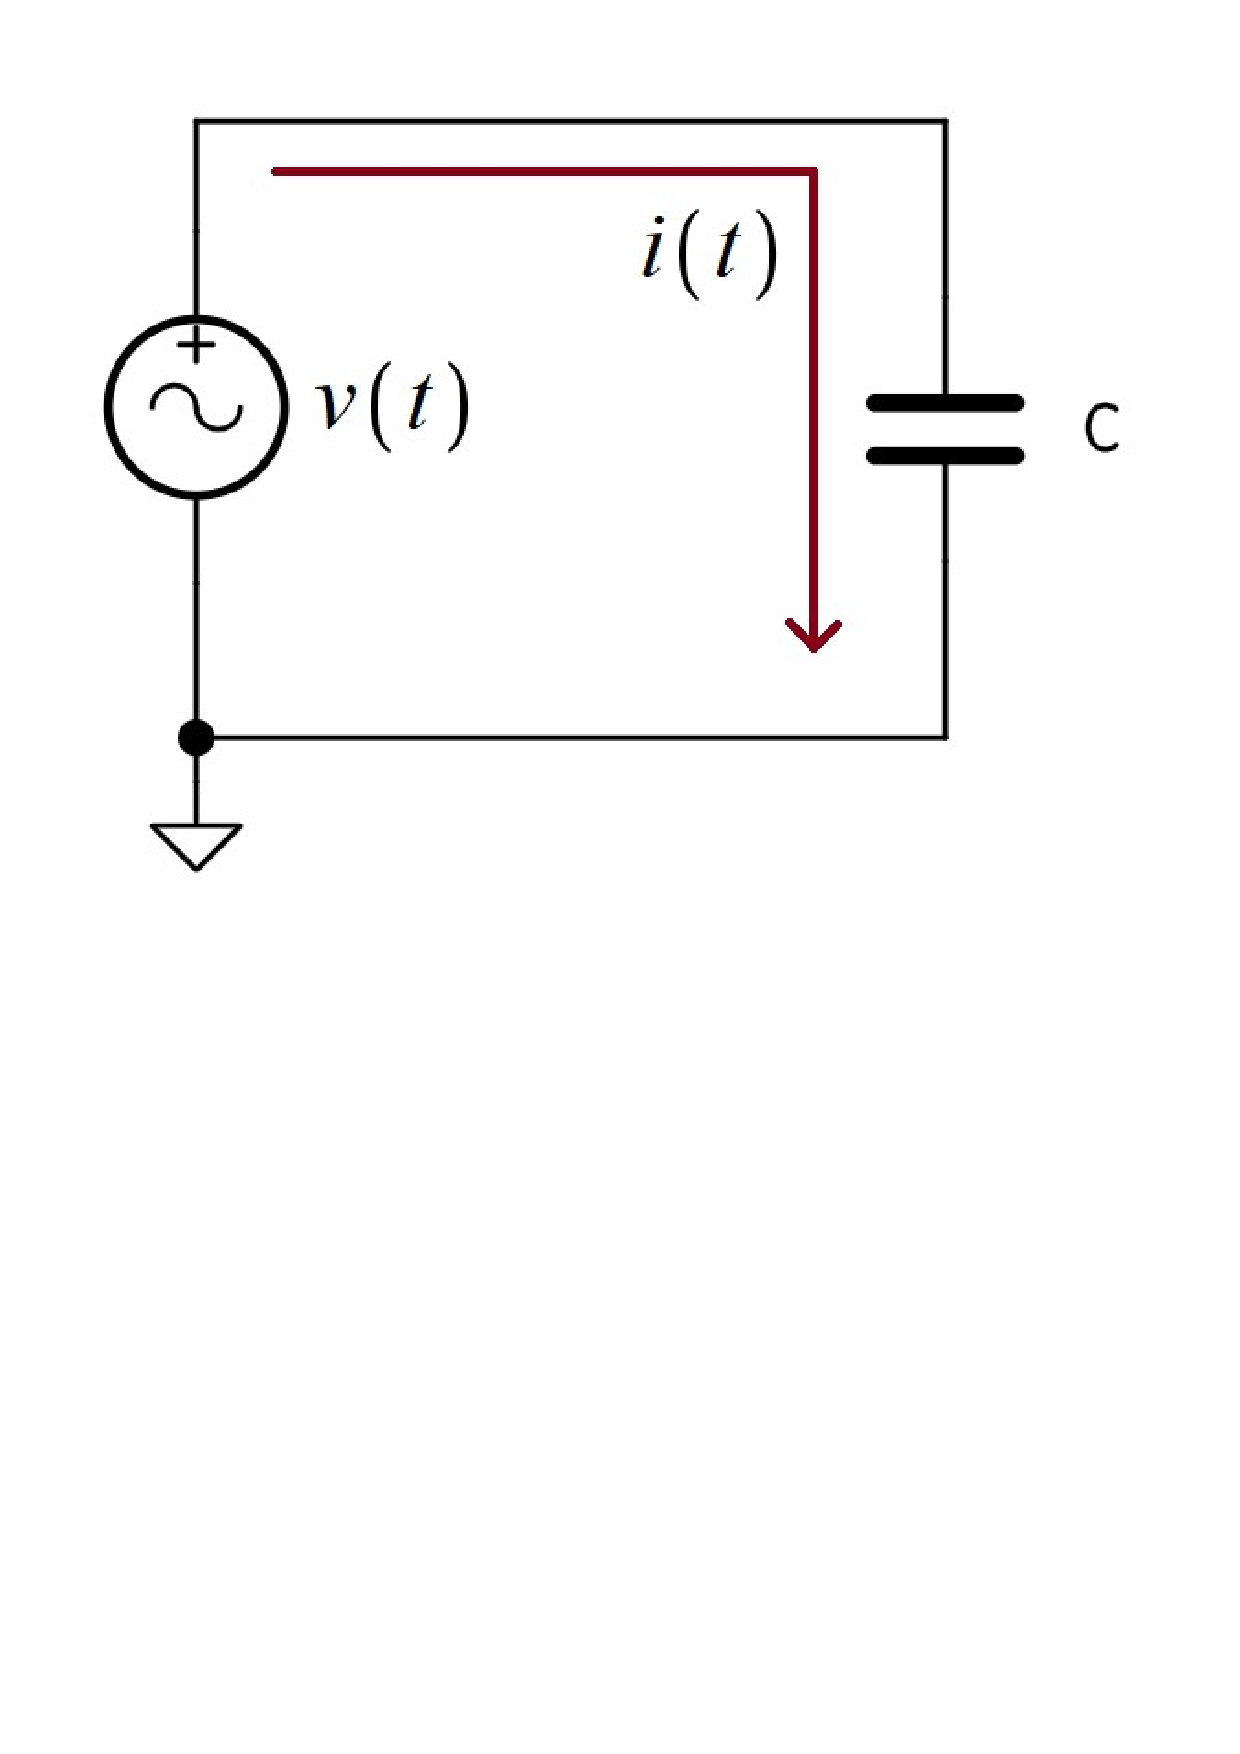
\includegraphics[clip, trim=0 400 0 0, width=0.60\textwidth]{Sections/4_TechnicalAnalysis/Figures/4_1_1_CapCircuit.pdf}
    \caption{An AC voltage source, $v(t)$, across a capacitor causes a current, $i(t)$, to flow through it.}
    \label{fig:4_1_1_CapCircuit}
\end{figure}

The current in the circuit is, because of the capacitor, as in eq \refq{eq:4_1_1_CapCurrent}.
\begin{equation}\label{eq:4_1_1_CapCurrent}
    i(t) = C\cdot\frac{d}{dt} (v(t))
\end{equation}
Transforming \refq{eq:4_1_1_CapCurrent} into the frequency domain with the laplace transform gives eq \refq{eq:4_1_1_CapCurrent2}.
\begin{equation}\label{eq:4_1_1_CapCurrent2}
    1
\end{equation}
